% Copyright (c) 2018 Alexander Bluhm <bluhm@genua.de>
%
% Permission to use, copy, modify, and distribute this software for any
% purpose with or without fee is hereby granted, provided that the above
% copyright notice and this permission notice appear in all copies.
%
% THE SOFTWARE IS PROVIDED "AS IS" AND THE AUTHOR DISCLAIMS ALL WARRANTIES
% WITH REGARD TO THIS SOFTWARE INCLUDING ALL IMPLIED WARRANTIES OF
% MERCHANTABILITY AND FITNESS. IN NO EVENT SHALL THE AUTHOR BE LIABLE FOR
% ANY SPECIAL, DIRECT, INDIRECT, OR CONSEQUENTIAL DAMAGES OR ANY DAMAGES
% WHATSOEVER RESULTING FROM LOSS OF USE, DATA OR PROFITS, WHETHER IN AN
% ACTION OF CONTRACT, NEGLIGENCE OR OTHER TORTIOUS ACTION, ARISING OUT OF
% OR IN CONNECTION WITH THE USE OR PERFORMANCE OF THIS SOFTWARE.

\documentclass[14pt]{beamer}
\usetheme{Frankfurt}
\usepackage{tikz}
\usetikzlibrary{shapes.geometric}
\author{Alexander Bluhm}
\title{OpenBSD Security Features}
\institute{genua GmbH\\ \url{bluhm@genua.de}\\ \url{bluhm@openbsd.org}}
\date{September 20, 2018}

\begin{document}

\begin{frame}
\titlepage
\end{frame}

\begin{frame}{Agenda}
\setcounter{tocdepth}{1}
\tableofcontents
\end{frame}

\section{kbind(2) System Call}

\subsection{Lazy Binding}
\begin{frame}{Lazy Binding}
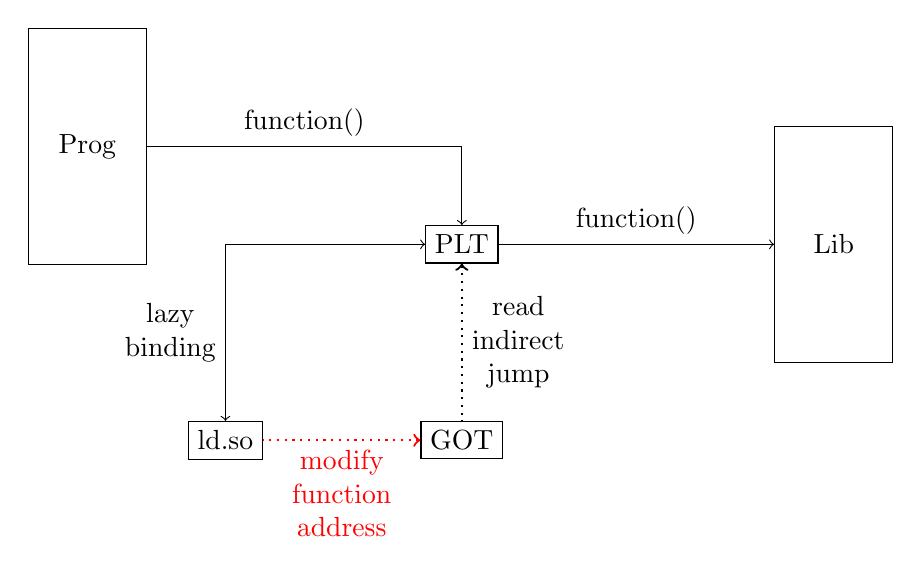
\begin{tikzpicture}
\draw
    node [draw,minimum height=3cm,minimum width=1.5cm] (prog) {Prog};
\draw (prog.east) [->] -- ++(4,0) node [midway,above] {function()} -- ++(0,-1)
    node [draw,below] (plt) {PLT};
\draw (plt.south) [<-,dotted,thick] -- ++(0,-2)
    node [midway,right,align=center] {read\\ indirect\\ jump}
    node [draw,solid,thin,below] (got) {GOT};
in ld.so \draw (got.west) [<-,dotted,thick,red] -- ++(-2,0)
    node [midway,below,align=center] {modify\\ function\\ address}
    node [draw,solid,thin,left,black] (ldso) {ld.so};
\draw (plt.west) [<->] -| 
    node [near end,left,align=center] {lazy\\ binding} (ldso);
\draw (plt.east) [->] -- ++(3.5,0) node [midway,above] {function()}
    node [draw,right,minimum height=3cm,minimum width=1.5cm] (lib) {Lib};
\end{tikzpicture}
\end{frame}

\subsection{Dangerous PLT GOT}
\begin{frame}{Dangerous PLT GOT}
\begin{itemize}
    \item Procedure Linkage Table
    \item Global Offset Table
    \item writeable table of code pointers
    \item mprotect(2) in ld.so is another gadget
\end{itemize}
\end{frame}

\subsection{Solution kbind(2)}
\begin{frame}{Solution kbind(2)}
\begin{itemize}
    \item modifies single GOT entry
    \item implicit atomic mprotect(2)
    \item can only called from ld.so(1)
    \item protected by data cookie
\end{itemize}
\end{frame}

\subsection{Questions}
\begin{frame}{Questions}
\begin{center}
\begin{tikzpicture}
\draw [font=\Huge] node {?};
\end{tikzpicture}
\end{center}
\end{frame}

\subsection{Links}
\begin{frame}{Links}
\url{https://www.openbsd.org/papers/bsdtw.pdf}
\url{https://www.technovelty.org/linux/plt-and-got-the-key-to-code-sharing-and-dynamic-libraries.html}
\end{frame}

\end{document}
